% 6 - 7  pages including all
\documentclass[a4paper,twoside]{article}

\usepackage{epsfig}
\usepackage{subfigure}
\usepackage{calc}
\usepackage{amssymb}
\usepackage{amstext}
\usepackage{amsmath}
\usepackage{amsthm}
\usepackage{multicol}
\usepackage{pslatex}
\usepackage{apalike}
\usepackage{SCITEPRESS}     % Please add other packages that you may need BEFORE the SCITEPRESS.sty package.


\subfigtopskip=0pt
\subfigcapskip=0pt
\subfigbottomskip=0pt

\begin{document}

\title{Dense Neural Networks for Secondary Structure Analysis of Biological Sequences}

\author{\authorname{Semyon Grigorev\sup{1,2}, Polina Lunina\sup{1,2}}
\affiliation{\sup{1}St. Petersburg State University, 7/9 Universitetskaya nab., St.Petersburg, Russia}
\affiliation{\sup{2}JetBrains Research, Universitetskaya emb., 7-9-11/5A, St.Petersburg, Russia}
\email{s.v.grigoriev@spbu.ru, Semen.Grigorev@jetbrains.com, lunina\_polina@mail.ru}
}

\keywords{Dense Neural Network, DNN, Machine Learning, Secondary Structure, Formal Grammar, Parsing}

\abstract
{
Abstract is very abstract. Abstract is very abstract. Abstract is very abstract.
Abstract is very abstract. Abstract is very abstract. Abstract is very abstract.
Abstract is very abstract. Abstract is very abstract. Abstract is very abstract.
Abstract is very abstract. Abstract is very abstract. Abstract is very abstract.
Abstract is very abstract. Abstract is very abstract. Abstract is very abstract.
Abstract is very abstract. Abstract is very abstract. Abstract is very abstract.
Abstract is very abstract. Abstract is very abstract. Abstract is very abstract.
Abstract is very abstract. Abstract is very abstract. Abstract is very abstract.
Abstract is very abstract. Abstract is very abstract. Abstract is very abstract.
}

\onecolumn \maketitle \normalsize \vfill

\section{\uppercase{Introduction}}
\label{sec:introduction}

\noindent Accurate sequences classification and subsequences detection are an open problems in different areas of bioinformatics, such as genomics and protenomics. 
Challenge here is a high variability of sequences which one want to mark as a same class.
For some type of sequences its secondary structure is a !!! and this fact may be used for !!!.

For example, algorithms that can efficiently and accurately identify and classify bacterial taxonomic hierarchy have become a focus in computational genetics.
The idea that secondary structure of genomic sequences is sufficient for solving the detection and classification problems lies at the heart of many tools~\cite{GrammarsRNA,PCFG,meta,LWPCFG}. 
The secondary structure can be specified in terms of formal grammars. 
The sequences obtained from the real bacteria usually contain a huge number of mutations and ``noise'' which renders precise methods impractical. 
Probabilistic grammars and covariance models (CMs) are a way to take the noise into account~\cite{EddyDurbin}.
For example, CMs are successfully used in the Infernal tool~\cite{Infernal}.
Neural networks is another way to deal with ``noisy'' data. 
The works~\cite{Humidor,ANN} utilize neural networks for 16s rRNA processing and demonstrate promising results.

In this work we propose the way to combine formal grammars and neural networks for secondary structure features processing.
The key idea is does not try to model full (sub)sequence of interest by grammar, but create grammar which describes features of secondary structure and use neural network for these features processing.

\section{\uppercase{Proposed solution}}
\label{sec:proposedSolution}

\noindent We propose to combine neural networks and ordinary context-free grammars (not probabilistic which are usually used in this area) in order to handle information of sequences' secondary structure. 
Namely, we propose to extract secondary structure features by using the ordinary context-free grammar and use the dense neural network for features processing.
Features can be extracted by any parsing algorithm and then presented as a boolean matrix but we choose parsing algorithm based on matrix multiplication.

In this section we describe all components of our recipe and provide some examples end explanations on it.
 
\subsection{Context-Free Grammars}

\noindent The first component is a context-free grammar. 
It is a well-known fact that secondary structure of sequence may be approximated by using formal grammars.
There is number of works that utilize this fact for different purposes~\cite{!!!!}.

Usually probabilistic context-free grammars are used for secondary structure modeling because it allows to dealt with variations (mutations or some kinds of noise).
In the opposite of it, we use ordinary (not probabilistic) grammars.
Our goal is not to model secondary structure of whole sequence (which required probabilistic grammars), but describe features of secondary structure, such as stems, loops, pseudoknots and it's composition.
The set of feature types is limited by class of the grammar which we use.
For example, pseudoknots can not be expressed by context-free grammars, but can be expresed by using cinjunctive~\cite{KanchanDevi2017,zier2013rna,Okhotin:2001:CG:543313.543323} or multiple context-free~\cite{SEKI1991191,Riechert:2016:ADP:2972703.2972851}.

The context-free grammar $G_0$ which we use in our experiments is presented in figure~\ref{fig:cfg-rna}.
It is a context-free grammar over four-letters in the alphabet $\Sigma=\{A,C,G,T\}$ with start nonterminal \verb|s1|.
This grammar which describes composition of stems with bounded minimal height.

\begin{figure}
\begin{verbatim}
s1: stem<s0> any

any_str : any*[2..10]

s0: any_str | any_str stem<s0> s0

any: A | T | C | G

stem1<s>: A s T | G s C | T s A | C s G 

stem2<s>: stem1< stem1<s> >

stem<s>:  
      A stem<s> T 
    | T stem<s> A 
    | C stem<s> G 
    | G stem<s> C 
    | stem1< stem2<s> >  
 } 
\end{verbatim}
\caption{Context-free grammar $G_0$ for RNA secondary structure features extraction}
\label{fig:cfg-rna}
\end{figure}

First of all, we provide a brief description of grammar specification language.
Left hand side and right hand side of rule are separated by the \verb|:| sign.
In the right hand side one can use extended regular expressions over union alphabet of terminals and nonterminals.
Such constructions as bounded repetition and alternative are available.
For example, \verb|any*[2..10]| is a bounded repetition and it is stands that nonterminal \verb|any| may be repeated any number of times from 2 up to 10.
Example of rule which uses alternatives is \texttt{any: A | T | C | G} which stands that \verb|any| is one of four terminals.

Another important feature of the language is parametric rules or metarules which allow one to create a reusable grammar templates.
More details on metarules one can find in~\cite{!!!}.
The example of metarule in our grammar is \texttt{stem1<s>: A s T | G s C | T s A | C s G}.
This rule has one parameter \verb|s| which stands for something that should be embedded into stem.
Application of this rule to \verb|any_str| allow one to define stem with loop of length from 2 up to 10.
In our grammar we use metarules in order to describe stems with bounded minimal height: \verb|stem1<s>| is a stem with height exactly 1,  \verb|stem2<s>| is a stem with height exactly 2, and \verb|stem<s>| is a stem with height not lower than 3.

Now we explain what does this grammar meens.
This grammar describe a recursive composition of stems.
To see it one can look at the rule for \verb|s0| which is recursive and shows that composition of stems may be embedded into stem (\verb |stem<s0>| in the right side of this rule).
Every stem should has height not lower then 3 and builds only from classical base pairs.
Stems may be connected by arbitrary sequence of length from 2 up to 10, and loops have the same length.
Graphical explanation of this description one can find in figure~\ref{fig:cfg-rna-graphical}.

\begin{figure}
\centering
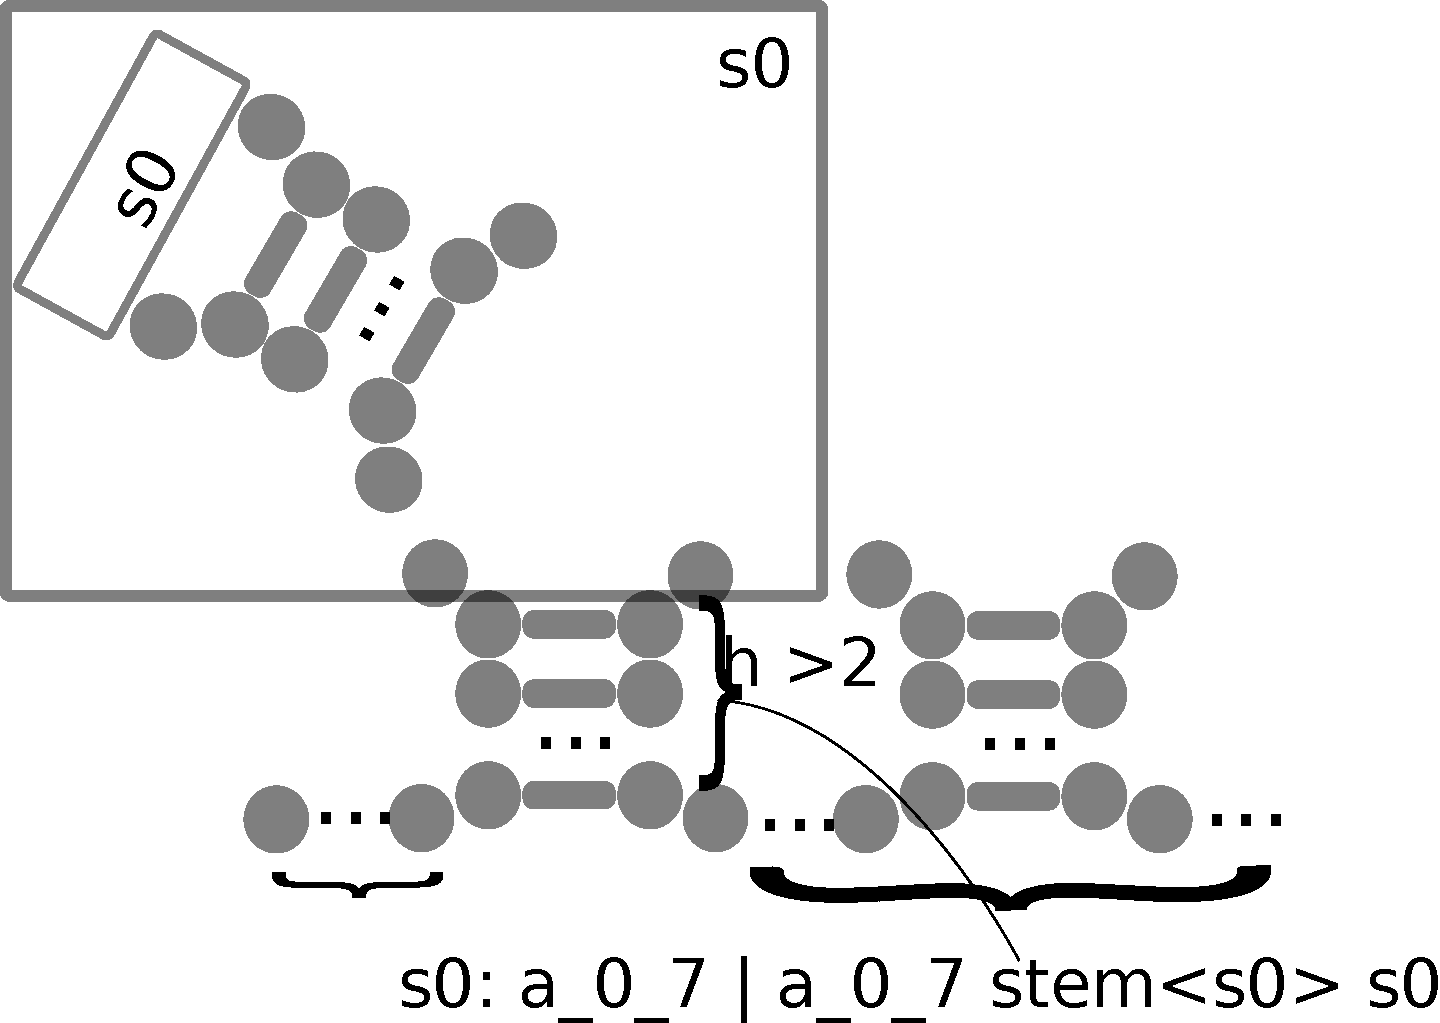
\includegraphics[width=.5\textwidth]{figures/16sgrammar.pdf}
\caption{Graphical explanation of pattern which is described by grammar in the figure~\ref{fig:cfg-rna}}
\label{fig:cfg-rna-graphical}
\end{figure}

Note that grammar is a variable parameter and may be tuned for specific cases.
For example, one can vary length of unfoldable sequence by changing rule for \verb|any_str|: \verb|any_str : any*[0..10]|, \verb|any_str : any*[1..8]|, or something else.
Also one can increase (or decrease for some reason) the minimal height of stem, or add some new features, such as pseudoknots, in the grammar (in case of usage of conjunctive grammars instead of context-free one).


\subsection{Parsing Algorithm}

\noindent Parsing is a feature extraction, so undirected parsing: we want to find all derivable substrings of given string for all nonterminals, not to check derivability of given string or find the most probably derivation.

CYK --- as a classical well-known algorithm.

Matrices.

Valiant~\cite{Valiant:1975:GCR:1739932.1740048} --- subcubic algorithm based on matrix multiplication.

Rustam~\cite{Azimov:2018:CPQ:3210259.3210264} --- generalization for graph. Theoretical time complexity is !!! than complexity of the Valiant's algorithm, but in practice these algorithm avoid machinery on submatrices manipulation and demonstrate better performance with simple implementation.

Sparse matrices, boolean, GPGPU, etc.

Matrix-based approach can be generalized to conjunctive and even boolean grammars~\cite{OKHOTIN2014101}, as far as to multiple context-free grammars~\cite{mcfgMatrices}, which can provide a base for more expressive features descriptions handling.

\subsection{Matrices}

\noindent The result of parsing is a set of square boolean matrices. 
Each matrix $M_N$ contains information of all substrings which can be derived from nontermnal $N$.
In the other word, $M_N[i,j]=1$ iff $N \Rightarrow^*_G w[i,j]$ where $w$ is the input sequence and $G$ is context-free grammar, and $N$ is a nonterminal.
Thus, result of parsing is a set of matrices: one matrix for each nonterminal form grammar.
For futher processing we can select nonterminals of interest.
For our case, for grammar $G_0$ we select matrix for nonterminal \verb|s1|.

The example of such matrix is provided in figure~\ref{fig:matrix-simple-stem}.
This matrix is a result of parsing of the sequence \\ \texttt{CCCCATTGCCAAGGACCCCACCTTGGCAATCCC} \\ w.r.t the grammar $G_0$.

\begin{figure}
\centering
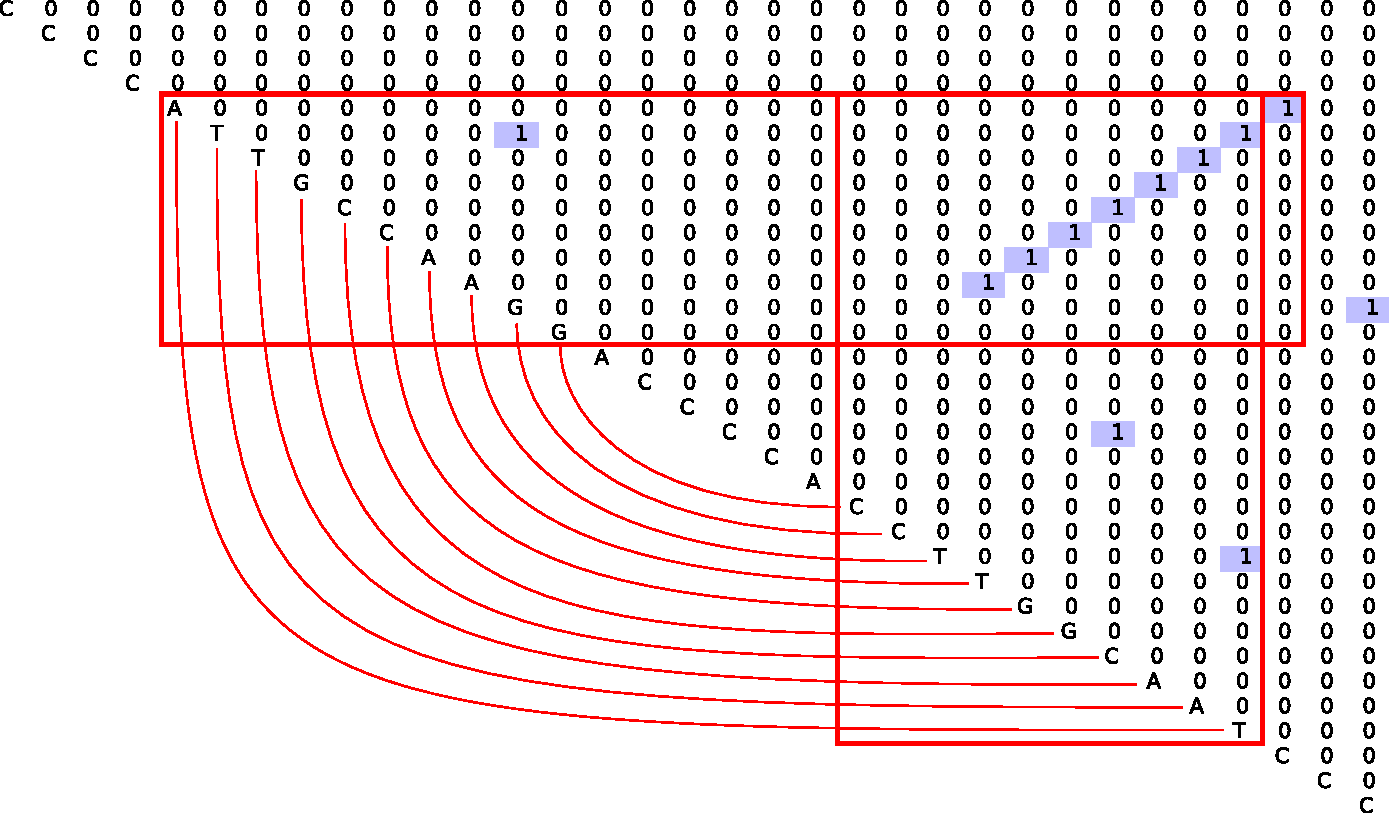
\includegraphics[width=.5\textwidth]{figures/4.pdf}
\caption{!!!!!}
\label{fig:matrix-simple-stem}
\end{figure}

Detailed description



Empty triangle can be omitted.
In order to handle matrices by using neural networks we vectorize it.
Row by row.
Complression to int or byte.
It is the reason why we want to try boolean networks.

\subsection{Neural Networks}

\noindent One of possible choice for classification.
Classical scenario is to provide features vectors and try to classify them which meens that network can select important features for each class.
In our case ht fact that ``$w[i,j]$ is derivable from nonterminal $N$'' which is encoded in the matrix is a feature.
So, matrix is a set (or vector) of features.

We use dense neural network because locality is broken during vectorization and any convolutions is inapplicable.

Current architecture and its motivation and explanation.
Huge dropout and batch normalization.

\subsection{Examples}
\label{sec:examples}

\noindent Here we provide more examples of matrices and point out some observations about it.

\begin{figure}
\centering
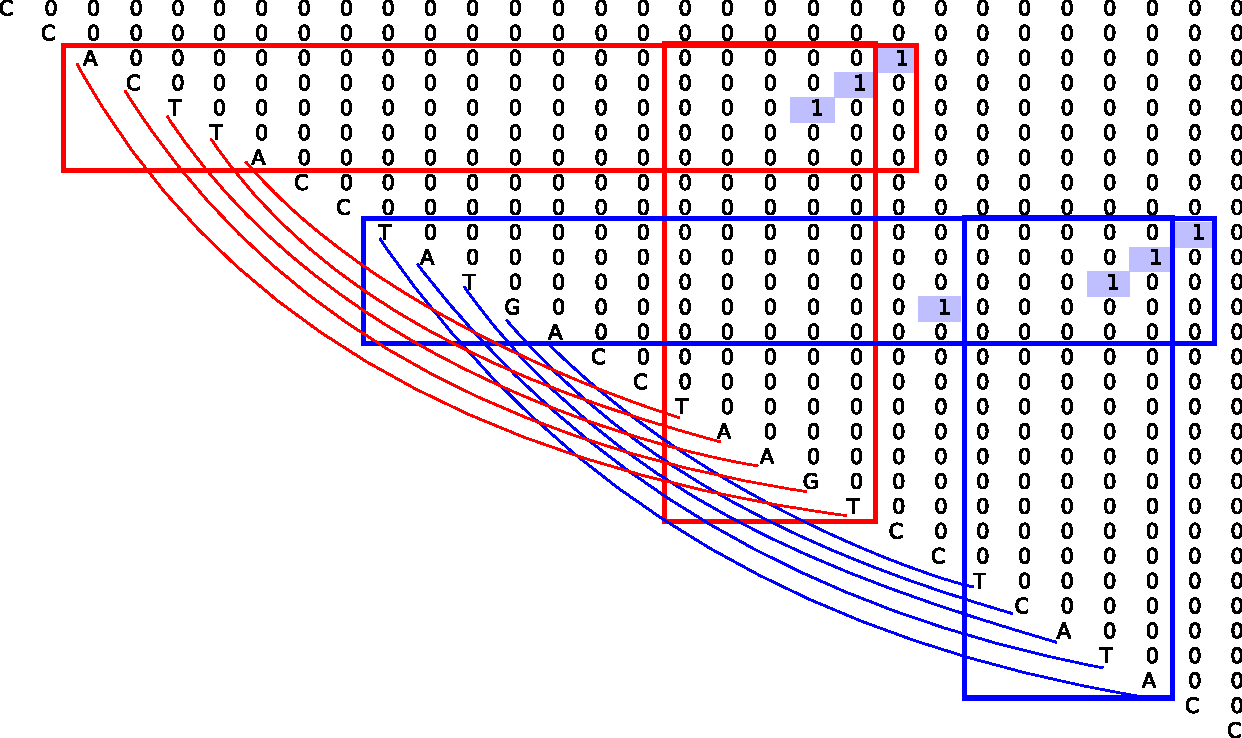
\includegraphics[width=.5\textwidth]{figures/5.pdf}
\caption{Parsing result for pseudoknot}
\label{fig:pseudoknot}
\end{figure}

First is observation about pseudoknots. 
Sequence: CCACTTACCTATGACCTAAGTCCTCATACC
As mentioned above, pseudoknots can not be expressed in terms of context-free grammars. 
But 
Blue and red
If newural network is powerful enough to !!! that these two fwetures should occurce simulatenously, then thay can detect pseudocnots.

The second is an example of matrix for real tRNA.
Sequence: CAGGGCATAACCTAGCCCAACCTTGCCAAGGTTGGGGTCGAGGGTTCGAATCCCTTCGCCCGCTCCA
Spec: Novosphingobium\_aromaticivorans\_DSM\_12444\_chr.trna57-GlyGCC (268150-268084)  Gly (GCC) 67 bp Sc: 22.97

Result of folding by tool!!!

\begin{figure}
\centering
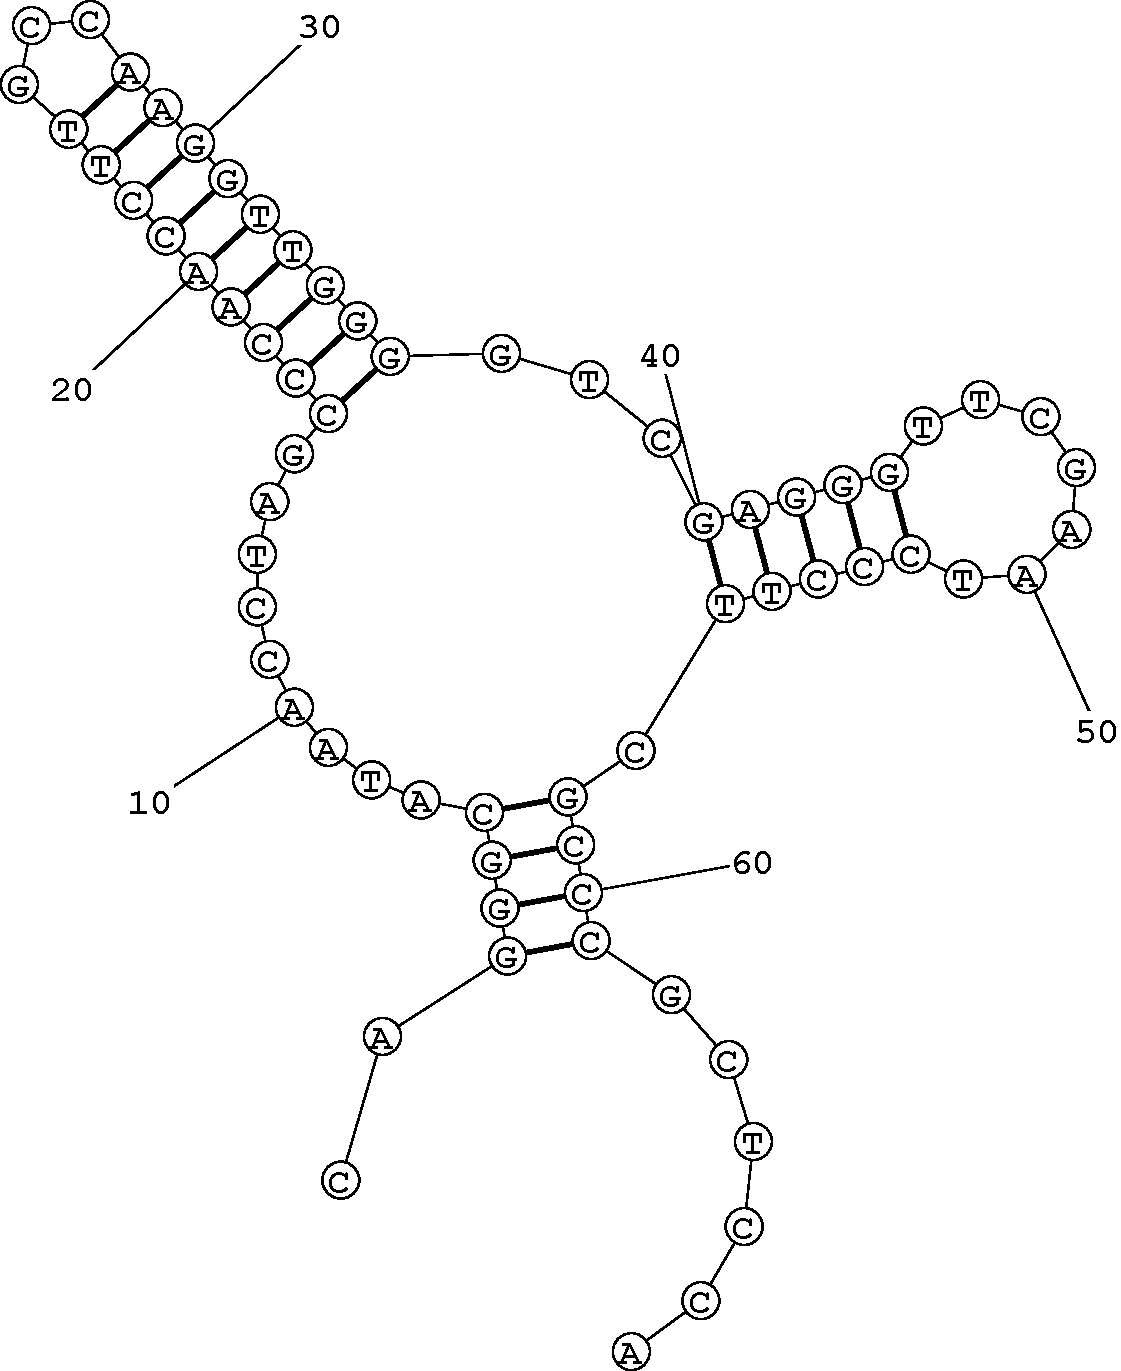
\includegraphics[width=.5\textwidth]{figures/Fold1.pdf}
\caption{!!!!!}
\label{fig:!!!}
\end{figure}


\begin{figure}
\centering
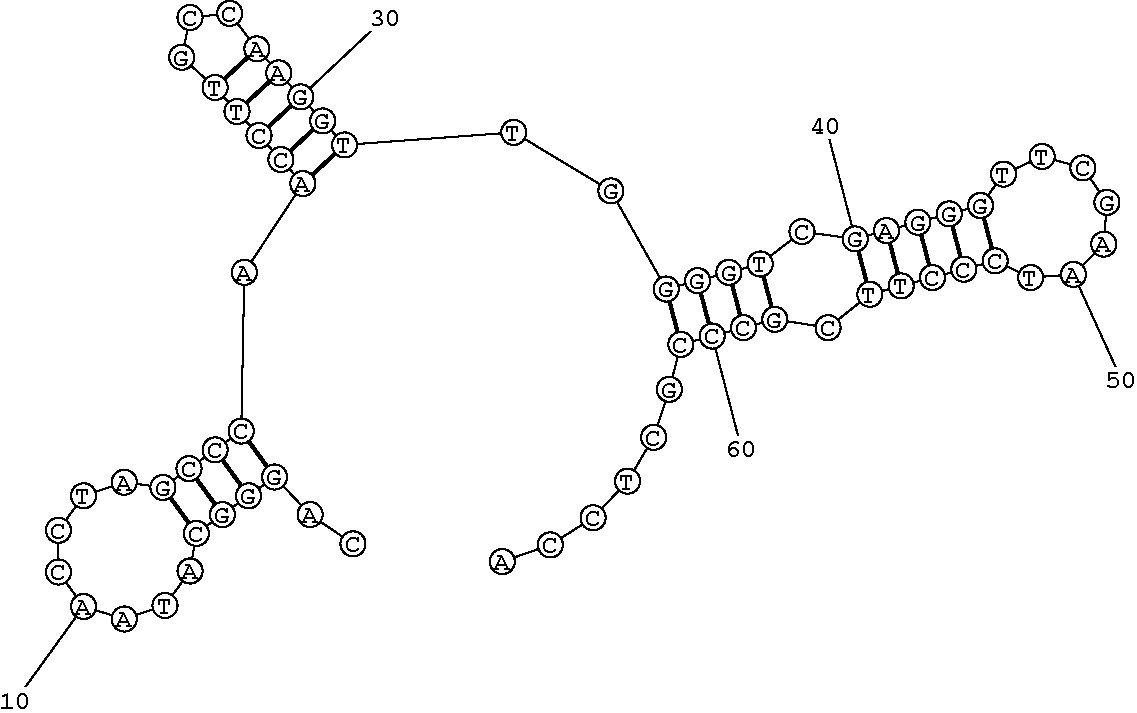
\includegraphics[width=.5\textwidth]{figures/Fold2.pdf}
\caption{!!!!!}
\label{fig:!!!}
\end{figure}


Matrix contains all these variants.
Blue and red boxes.
And some additional.

\begin{figure*}
\centering
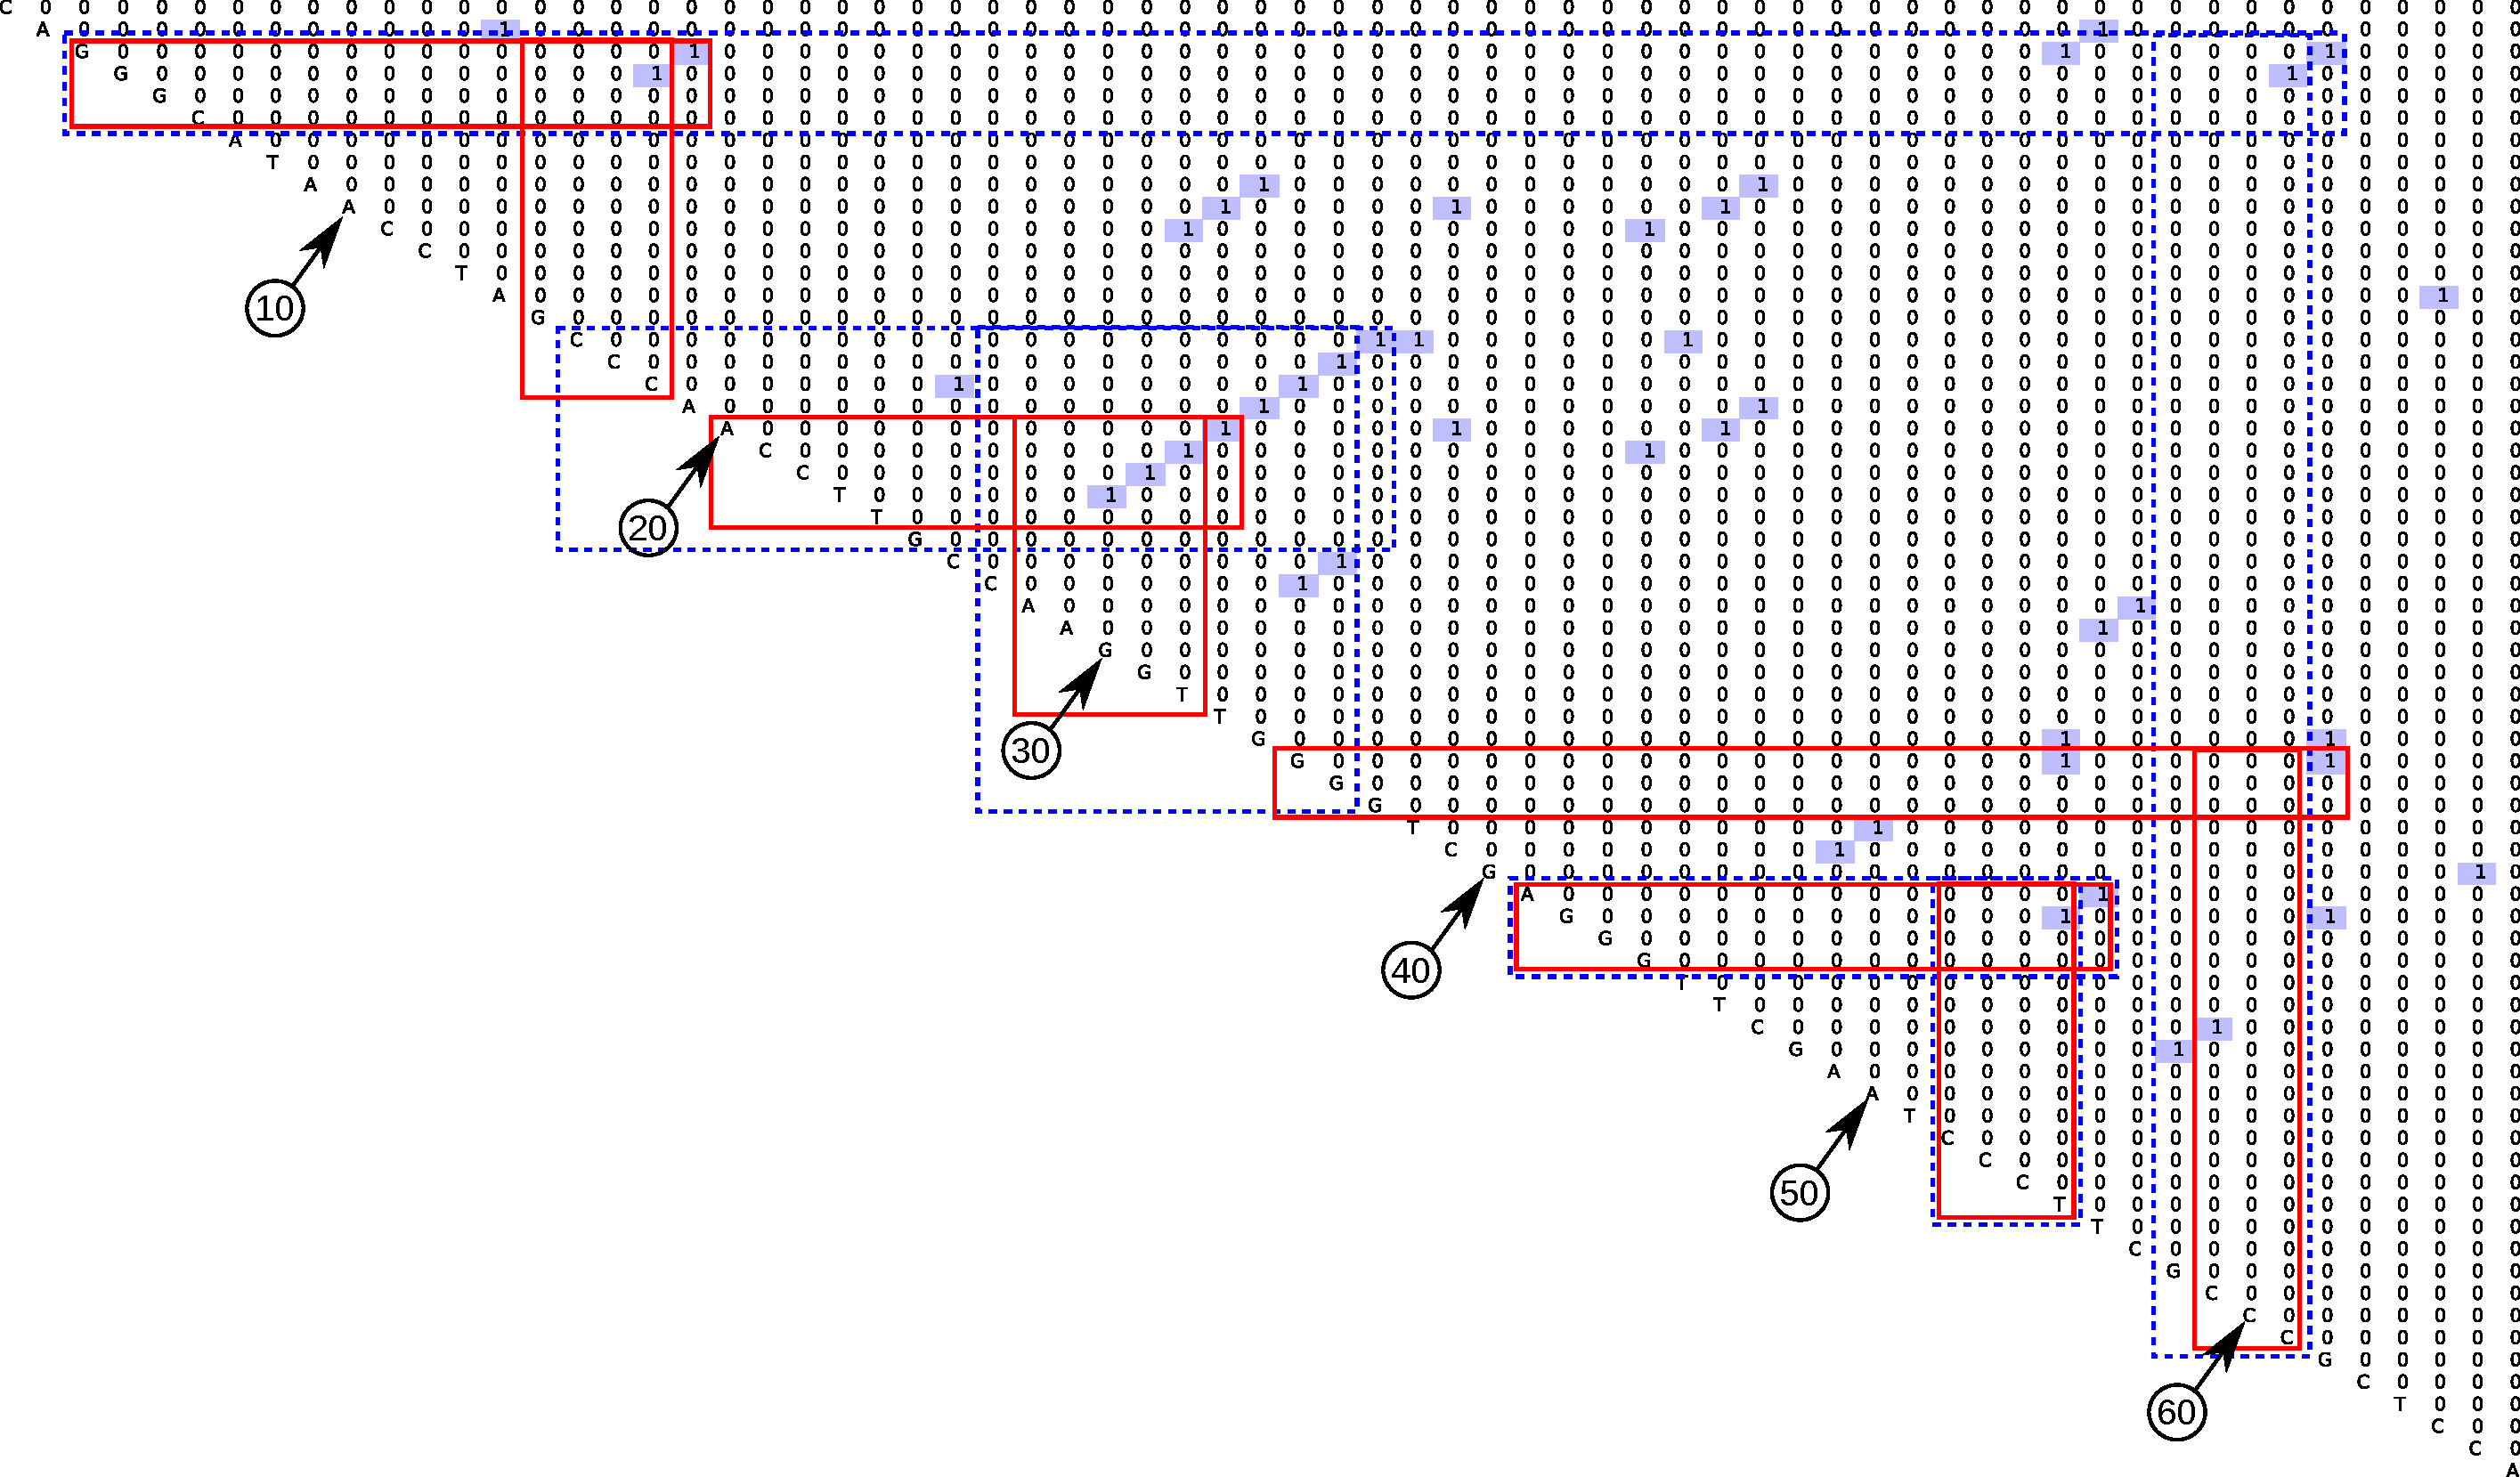
\includegraphics[width=.98\textwidth]{figures/0m.pdf}
\caption{!!!!!}
\label{fig:!!!}
\end{figure*}

Nontrivial compositions may be detected.
May we use NNs for secondary structure prediction?


\section{\uppercase{Evaluation}}
\label{sec:evaluation}

Two cases. 
16s rRNA and tRNA.

\noindent We evaluate the proposed approach for 16s rRNA detection.
We specify context-free grammars which detect stems with the hight of more than two pairs and their arbitrary compositions.
For network training we use dataset consisting of two parts: random subsequences of 16s rRNA sequences from the Green Genes database~\cite{pmid16820507} form positive examples, while the negative examples are random subsequences of full genes from the NCBI database~\cite{pmid19854944}.
All sequences have the length of 512 symbols, totally up to 310000 sequences.
After training, current accuracy is 90\% for validation set (up to 81000 sequences), thus we conclude that our approach is applicable.

Description of evaluation on tRNA classification.
Procariot --- eucarion.
500000 sequences.
Upper bound of length.
Results!!!

\section{\uppercase{Future Work}}
\label{sec:FutureWork}

\noindent The presented is a work in progress. 
The ongoing experiment is finding all instances of 16s rRNA in full genomes.
Also we plan to use the proposed approach for the filtration of chimeric sequences and the classification.
Composition of our approach with other methods and tools as well as grammar tuning and detailed performance evaluation may improve the applicability for the real data processing.


\section{\uppercase{Discussion}}
\label{sec:Discussion}

Protenomics (Witold Dyrka)~\cite{DBLP:Witold:Proteins}
More complex grammar: more symbols in alphabet, more complex featres.
More powerful languages required.
One of the possible crutial problem is functionally equivalence sequences with different length in protenomics.

Different lengths. Is a problem.
How can we normalize input?

Construct network which can handle sequences, not parsing data.
It may help to create an embedding.
It may be done by the next way.
\begin{enumerate}
\item Build and train the network which handle vectorized matrices.
\item Extend this network with head which should convert sequence to !!!
\item Train. Weights of first network is fixed.
\item For concrete problem we can tune weights for full network after second trained to appropriate quality.
\end{enumerate}

Other types of NNs.
Binary, convolutional (try to process matrix as a picture).
Pictures: problem with size, typical matrix size is big.

Prblems with data: how to create balanced set for training.
Datasets (like GreenGenes) contains huge nomder of samples for some well-studied organisms and very small number of samples for other.

Huge amount of experiments in different directions.
Plans should be discussed with community.


\section*{\uppercase{Acknowledgements}}

\noindent The research was supported by the Russian Science Foundation grant 18-11-00100 and a grant from JetBrains Research.


\vfill
\bibliographystyle{apalike}
{\small
\bibliography{example}}


\vfill
\end{document}

